\documentclass[11pt, xcolor=table]{beamer}
\usetheme{Singapore}

\usepackage[utf8]{inputenc}
\usepackage[T1]{fontenc}
\usepackage{soul}
\usepackage{graphicx}
\usepackage[normalem]{ulem}
\useunder{\uline}{\ul}{}

\graphicspath{{../../Figures/}}

\def\et{{\it et al.}}


\author{Cody Glickman  \\ CPBS Update Talk}

\title{Backups}

%\subtitle{}
%\logo{}

\date{ 
\includegraphics[height=2cm, width=2cm]{lablogo.png} \\ Nov 12th, 2018}
%\subject{}
\setbeamercovered{transparent}
\setbeamertemplate{navigation symbols}{}
\setbeamertemplate{theorems}[numbered]

\begin{document}
	\maketitle

  %------------------------------------------------------------------ Outline
	\begin{frame}{Research Update Outline}
	\begin{block}{Virulence Factors in Bacteriophages}
	In preperation
	\end{block}
	
	\begin{block}{Building Up Domains: Lysogenic Host Discovery}
	Incorporated into large collaborative NCBI initative
	\end{block}

	\begin{block}{Hybrid Viral Contig Prediction}
	In Preperation
	\end{block}
	\end{frame}
	%------------------------------------------------------------------
	\begin{frame}{Progress of Other Projects}
	\begin{block}{Asthma Environmental Microbiome}
	Submitted abstract to ATS
	\end{block}
	
		
	\begin{block}{Clinical NTM Gene Databases}
	Submitted ...
	https://mra.asm.org/latest 
	\end{block}
	
	\begin{block}{Duobiome: 18S/16S Parallel Analysis}
	In progress
	\end{block}
	
	
	\begin{block}{Genomic Retrieval and Blast Database Creation}
	Accepted Poster ISME 2018
	\end{block}
	
	\begin{block}{Hawaiian Soil Chemistry and Culture}
	Submitted ...
	\end{block}
	

	\end{frame}
	%-----------------------------------------------------------
\section{}


	\begin{frame}{Nontuberculous Mycobacterial (NTM) Infections}
	  
		\begin{block}{Number of Cases}
		The number of NTM cases is estimated over 100K
		\end{block}
		
		\begin{block}{Increasing Case}
		The rate of cases is estimated to grow at 8\% every year
		\end{block}
		
		
		\begin{block}{Populations at risk of developing NTM}
		\begin{itemize}
		\item Immunocompromised individuals 
		\item Patients with lung damage or malfunction 
		\item Residents of warm costal areas especially Hawaii
		%\item The Elderly 
		\end{itemize}
		\end{block} 
		
		\begin{block}
		
		\end{block}
	\vspace{-1cm}
	\tiny{Strollo SE, et al. Ann Am Thorac Soc. 2015 \\
	Adjemian J, et al. Am J Respir Crit Care Med. 2012}
	
	\end{frame}
	%----------------------------------------------------------
	% \begin{frame}{Laboratory Research Methods}
	% \begin{block}{Conditions for NTM Environmental Growth}
	% Identifying important characteristics for NTM growth 
	% \end{block}
	% 
	% \begin{block}{Environmental Microbiome}
	% Developing methods to characterize patient environments
	% \end{block}
	% 
	% \begin{block}{Clinical NTM}
	% \begin{itemize}
	% \item Developing resources to study clinical NTM
	% \item Identifying potential mechanisms of NTM transmission
	% \end{itemize}
	% \end{block}
	% 
	% 
	% \end{frame}
	
	%-----------------------------------------------------------
	\begin{frame}{Viral Focus}
	\begin{columns}
	\column{0.5\textwidth}
	\begin{block}{Bacteriophages (Phages)}
	Phages are DNA viruses that infect prokaryotes
	\end{block}
	
	\begin{block}{Phage Diversity}
	Investigating how phage abundance and diversity affect susceptibility to NTM lung infection
	\end{block}
	
	\begin{block}{Phage Vectors}
	Researching how phages act as carriers of bacterial genes within clinical NTM infections
	\end{block}
	
	
	\column{0.5\textwidth}
	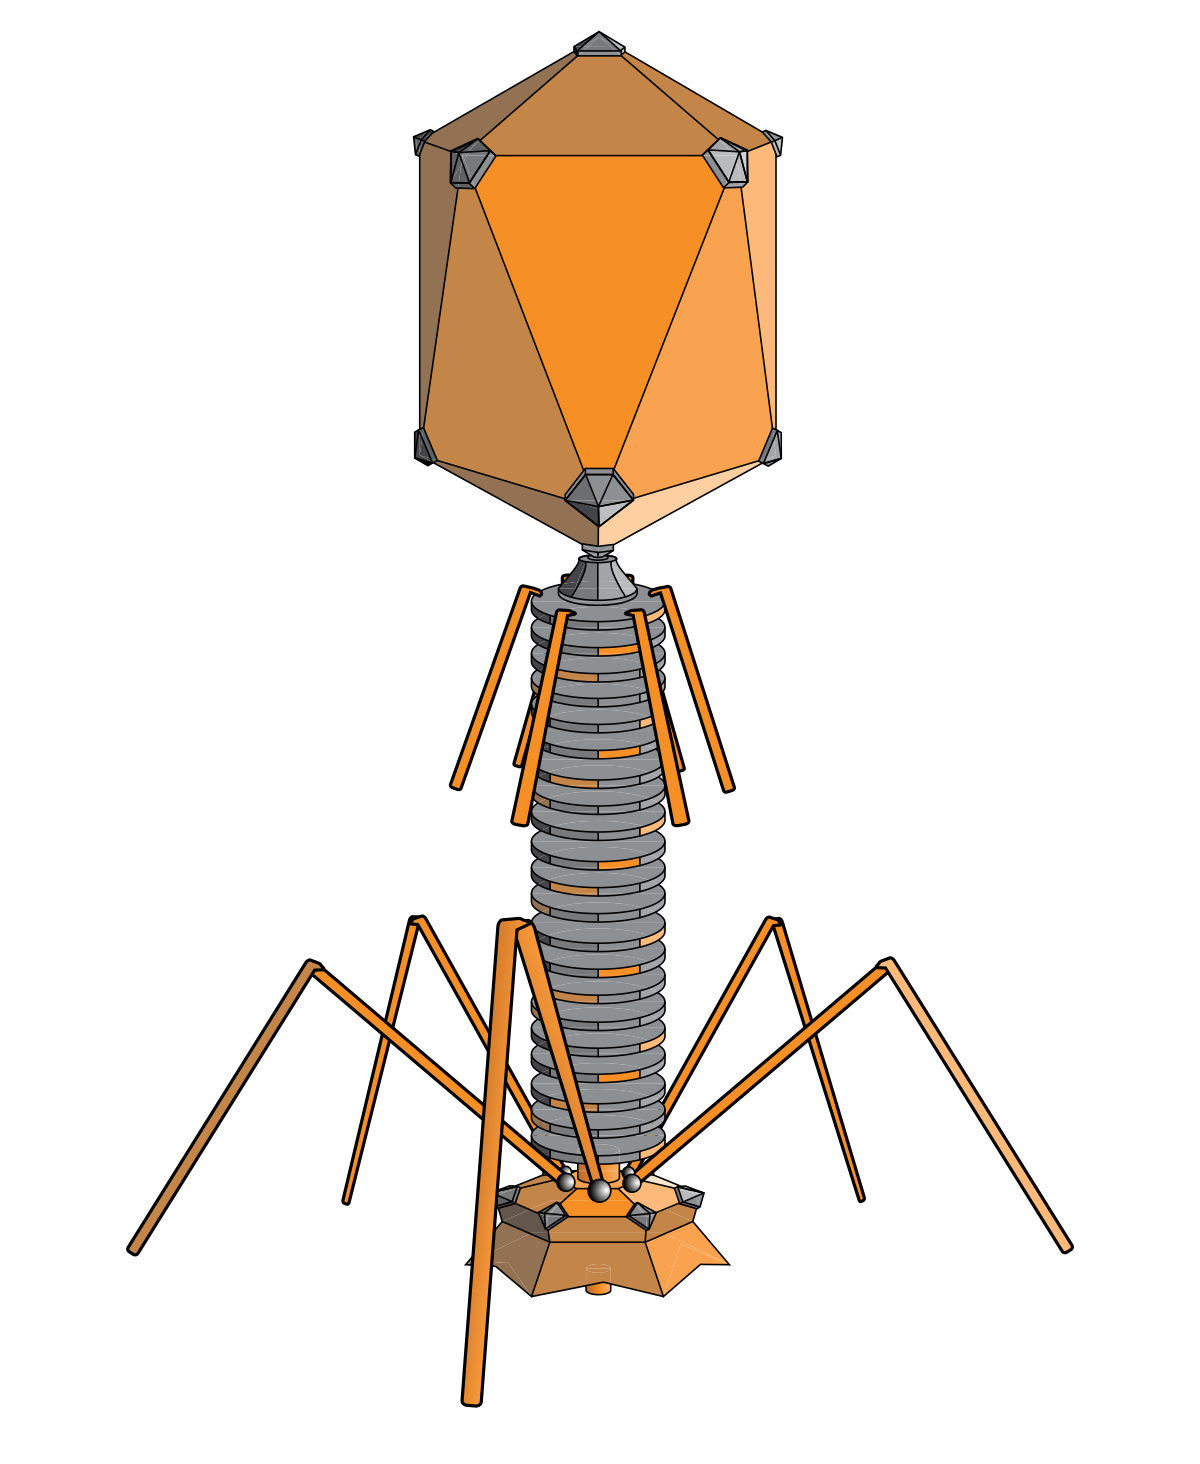
\includegraphics[height=5.5cm, width=5cm]{phage.png} \\
	\end{columns}
	
	
	\end{frame}
	%-----------------------------------------------------------

\section{Clinical NTM Gene Databases}
\subsection{}
	\begin{frame}{Species Identification of NTM at NJH}
  \begin{block}{Clinical NTM Gene Database}
  Developed updated database to characterize clinical NTM
  \end{block}
	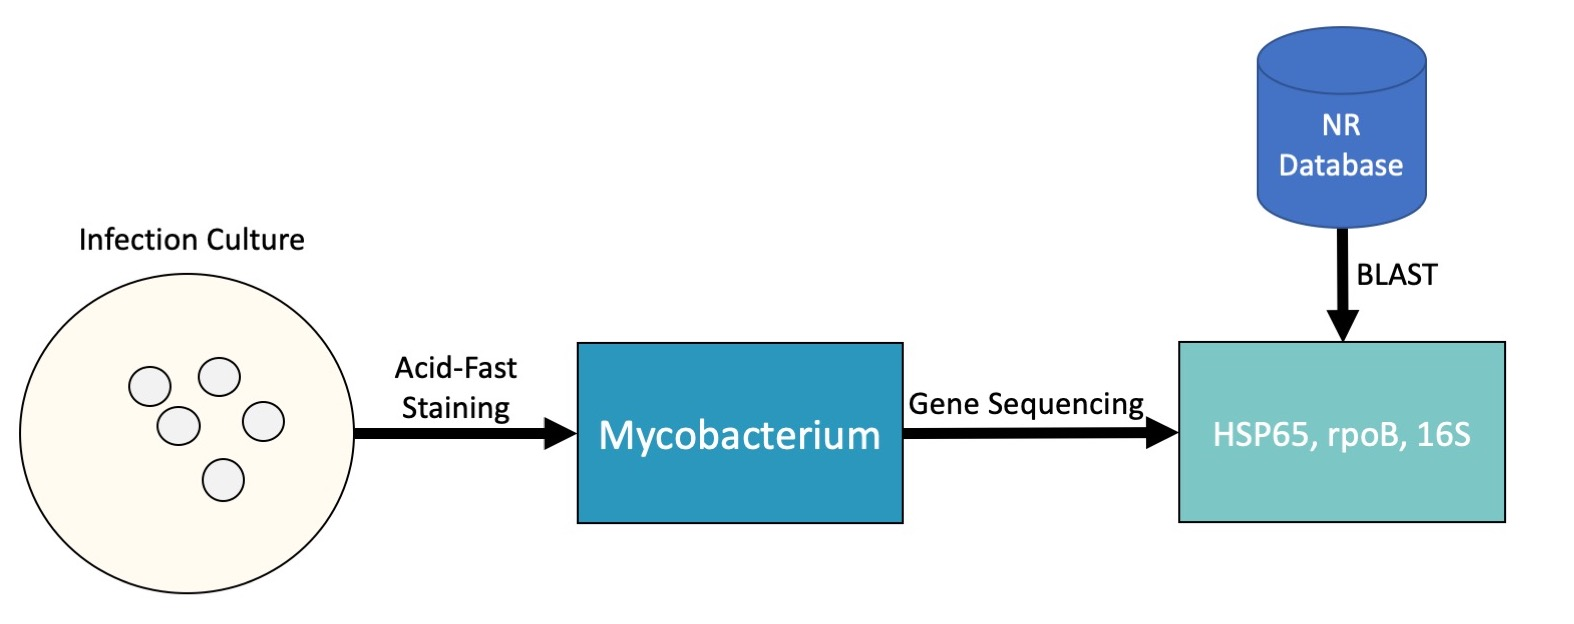
\includegraphics[height=5cm, width=11cm]{CPBS_11_18/NJH_Protocol.jpg}
	
	\end{frame}
	%-----------------------------------------------------------
	\begin{frame}{Limitations of Current Methods}
	
	\begin{columns}
	\column{0.5\textwidth}
	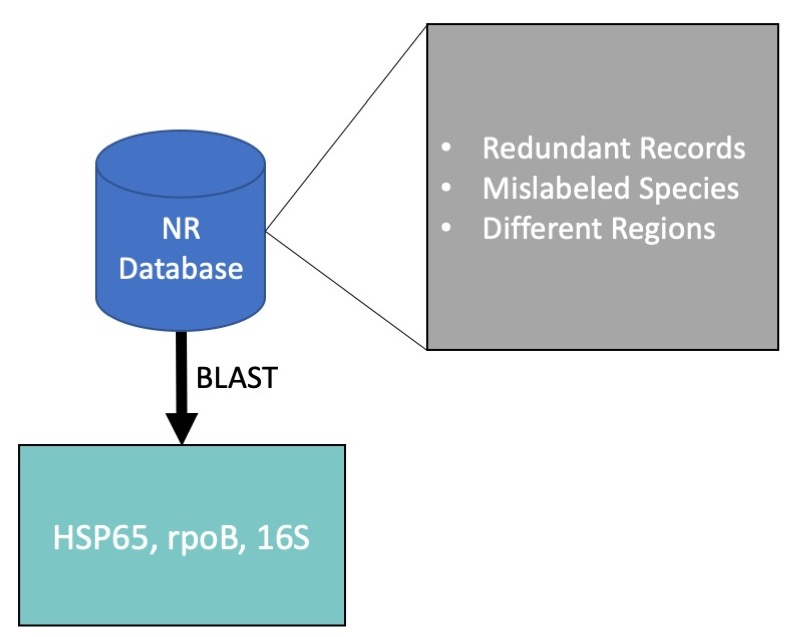
\includegraphics[height=5cm, width=5.5cm]{CPBS_11_18/Issues.jpg}
	\column{0.5\textwidth}
	\begin{block}{Redundant Records}
	Sequences between species are indistinguishable at the gene level
	\end{block}
	\begin{block}{Mislabeled Species}
	Naming conventions are constantly updated
	\end{block}
	\begin{block}{Different Regions}
	Current protocols amplify a specific region of gene
	\end{block}
	\end{columns}
	
	%\tiny{Sczyrba, A., et al. Nature Methods 2017}
	\end{frame}
	%-----------------------------------------------------------
  \begin{frame}{Curated Gene Databases}
  Line probe to determine Mycobacterial status (rpoB amplification)
  Mycobacteriology lab depends on targets for sequencing
  Creating a more efficent database
  \begin{block}{Number of Sequences per Species}
  Currenlty only two sequences per species are deposited into curated database
  \end{block}
  \center
  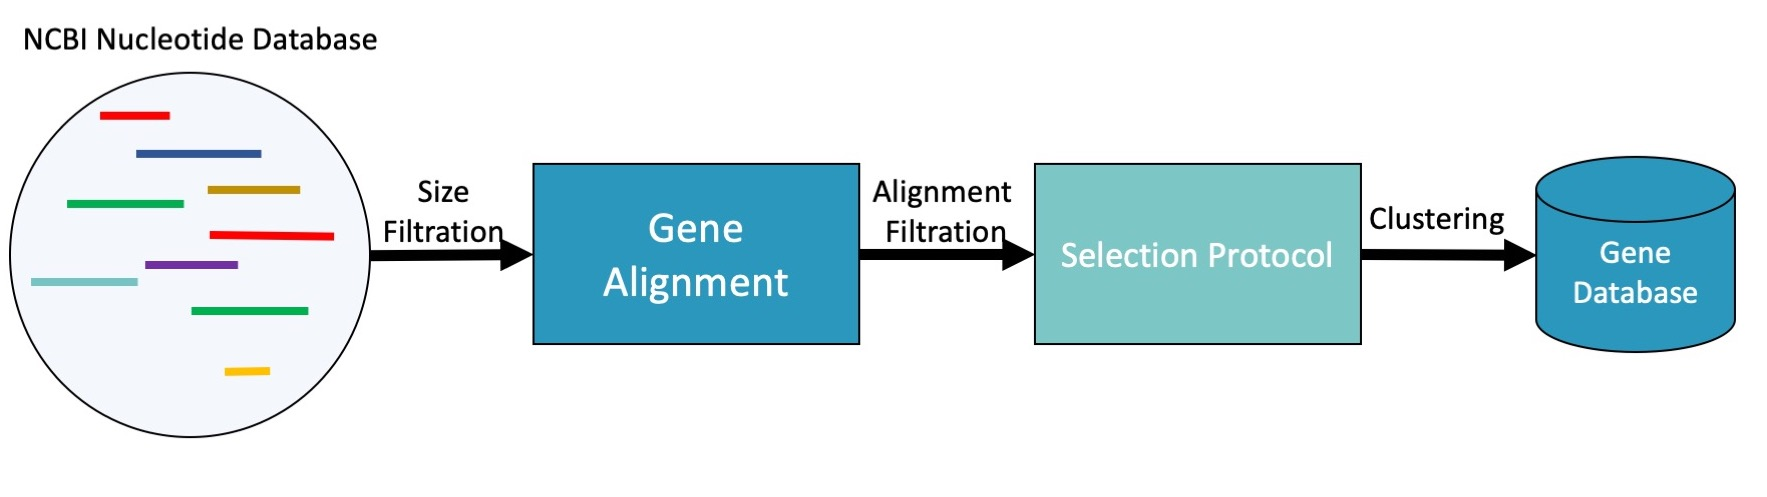
\includegraphics[height=4cm, width=11cm]{CPBS_11_18/Gene_Database_Workflow.jpg}
  \end{frame}


%-----------------------------------------------------------
  \begin{frame}{Selection Protocol}
  \center
  Culture Collection, internationally recognized strains, deposited in multiple locations
  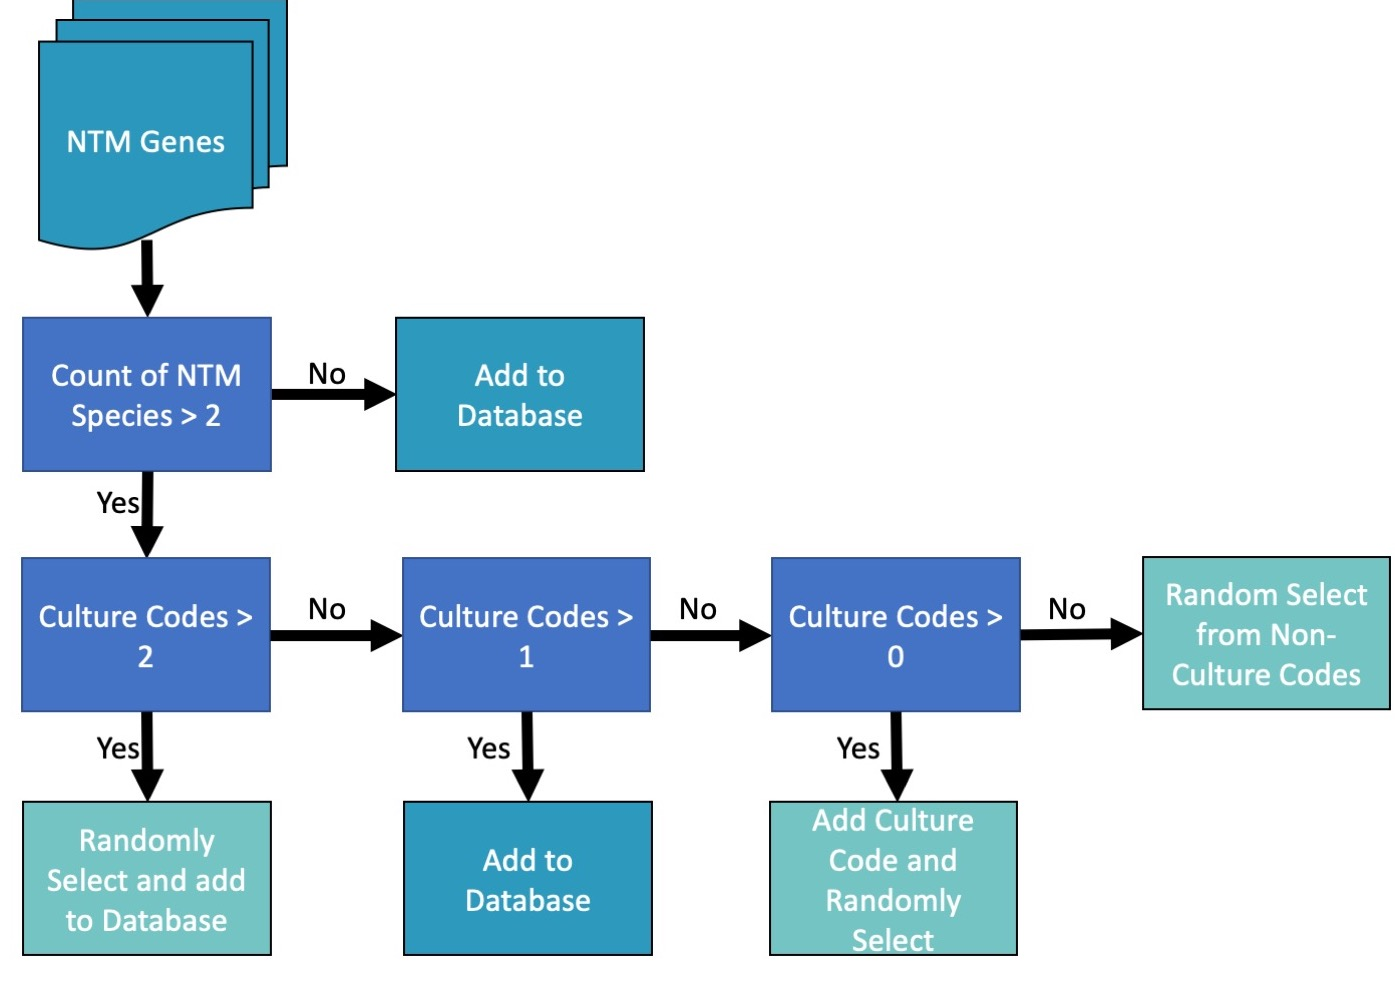
\includegraphics[height=7cm, width=11cm]{CPBS_11_18/Selection_Protocol.jpg}
  \end{frame}
%-----------------------------------------------------------
  \begin{frame}{Clinical Gene Databases}
  \begin{table}[]
  \begin{tabular}{|l|l|l|}
  \hline
  {\ul \textbf{Gene}} & {\ul \textbf{Region Size}} & {\ul \textbf{Unique Species}} \\     \hline
  hsp65 & 382 bases & 185 \\ \hline
  rpoB & 657 bases & 134 \\ \hline
  16s rRNA & 1470 bases & 184 \\ \hline
  \end{tabular}
  \caption{Table 1 highlights the regions lengths and size of the respective databases}
  \label{Test_Table}
  \end{table}
  \begin{block}{Species Overlap}
  107 species overlap between all three databases
  \end{block}
  \end{frame}
%-----------------------------------------------------------
	\begin{frame}{Database Validation}
	\vspace{-0.3cm}
	\begin{block}{hsp65}
	how many species: 197 documented species: Actual species counts remove clusters
	156 full length hsp65 genes compared against the hsp65 database
	\begin{itemize}
	\item 151/156 (96.73\%) returned the exact species
	\item 2/5 are in the top 5 hits \& 2/5 missing from database
	\end{itemize}
	\end{block}
	\vspace{-0.3cm}
	\begin{block}{Tree Comparison}
	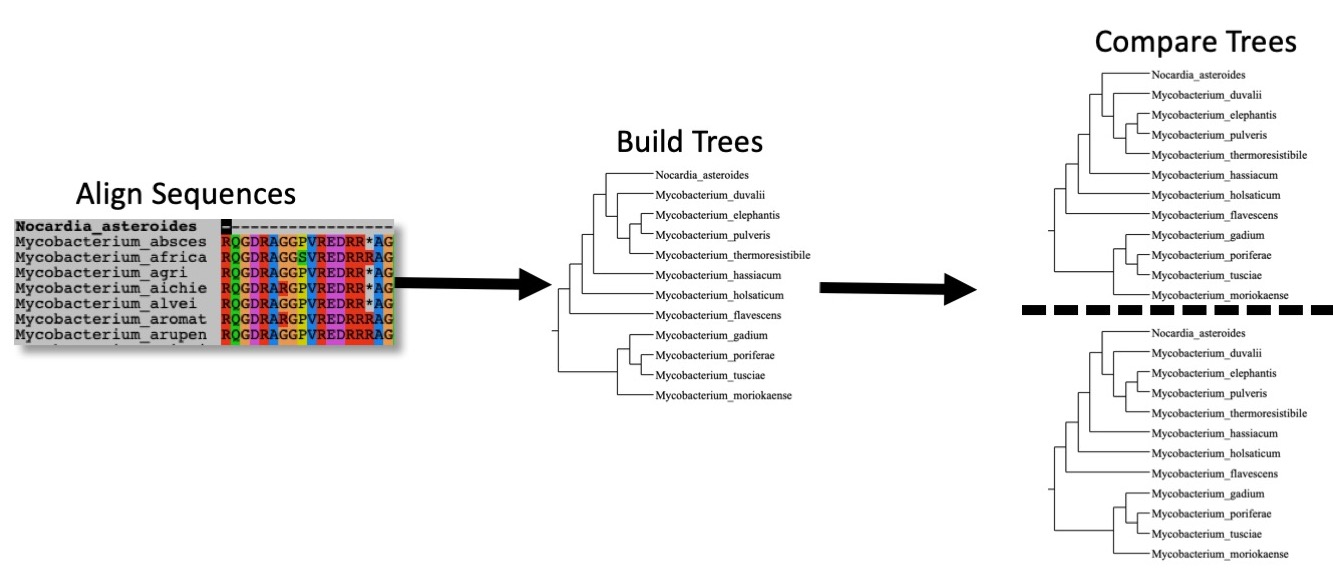
\includegraphics[height=4cm, width=11cm]{CPBS_11_18/Pipeline_Tree.jpg}
	\end{block}
	\vspace{-0.3cm}
	\begin{table}[]
  \begin{tabular}{|l|l|l|l|l|l|}
  \hline
  {\ul \textbf{E.Size}} & {\ul \textbf{nRF}} & {\ul \textbf{RF}} & {\ul \textbf{maxRF}}   & {\ul \textbf{scr-br}} & {\ul \textbf{ref-br}} \\ \hline
  153 & 0.90 & 220 & 244 & \cellcolor[HTML]{FCFF2F}0.59 & \cellcolor[HTML]{F8FF00}{\color[HTML]{000000} 0.61} \\ \hline
  \end{tabular}
  \end{table}
	
	\tiny{Dai, J, et al. J Clin Microbiol. 2011}
	\end{frame}
	

	%-----------------------------------------------------------
	\begin{frame}{rpoB-hsp65 Tree}
	rings around edges and lines for colors
	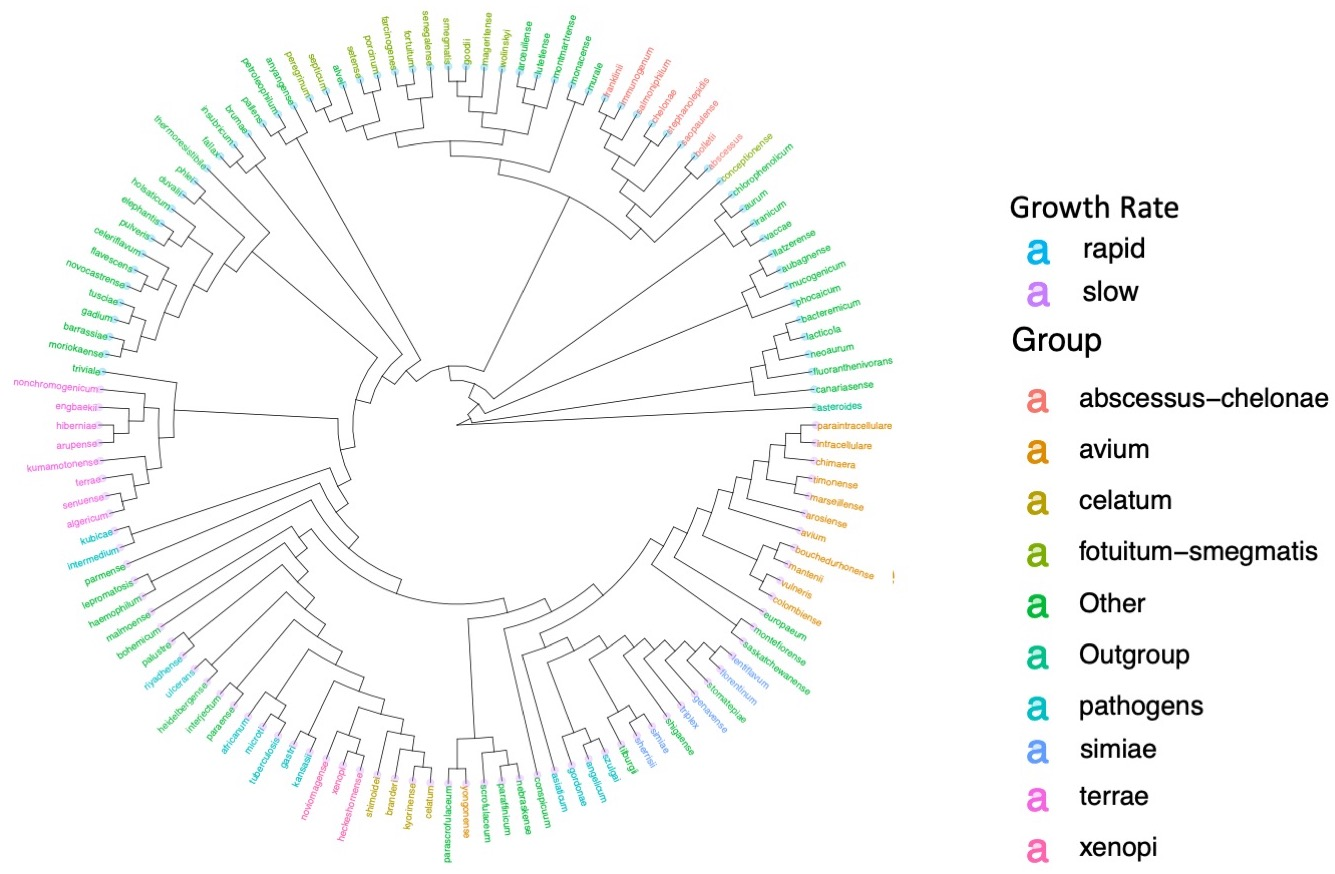
\includegraphics[height=8cm, width=11cm]{CPBS_11_18/Tree2.jpg}
	\end{frame}

%-----------------------------------------------------------
	\begin{frame}{Conclusions and Future Directions}
	
	\begin{block}{Representation}
	The subsetted databases are highly representative of prior published works
	\end{block}
	
	\begin{block}{Benefits of Curated Database}
	\begin{itemize}
	\item Aligned sequences to shared region
	\item Preferentially selected established culture codes
	\item Condensed and explicitly labeled ambiguous sequences 
  \end{itemize}
	\end{block}
	
	\begin{block}{Limitations}
	Size of the gene regions in databases may not differentiate between species or subspecies in this version
	\end{block}
	
	\tiny{Dai, J, et al. J Clin Microbiol. 2011 \\ Tortoli, E, et al. Infections, Genetics, and Evolution 2017}
  \end{frame}
%-----------------------------------------------------------

\section{Duobiome}
\subsection{}

	
	\begin{frame}{Microbiome}
	\begin{columns}
	\column{0.5\textwidth}
	\begin{block}{16S Ribosomal RNA Sequencing}
	\begin{itemize}
		\item Amplifies a region of gene
		\item Community level analysis 
	\end{itemize}
	\end{block}
		
		
	\begin{block}{Traditional Limitations}
	\begin{itemize}
		\item Multiple copies of 16S
		\item \alert{Prokaryotic specific}
	\end{itemize}
	\end{block}
	
	\column{0.5\textwidth}
	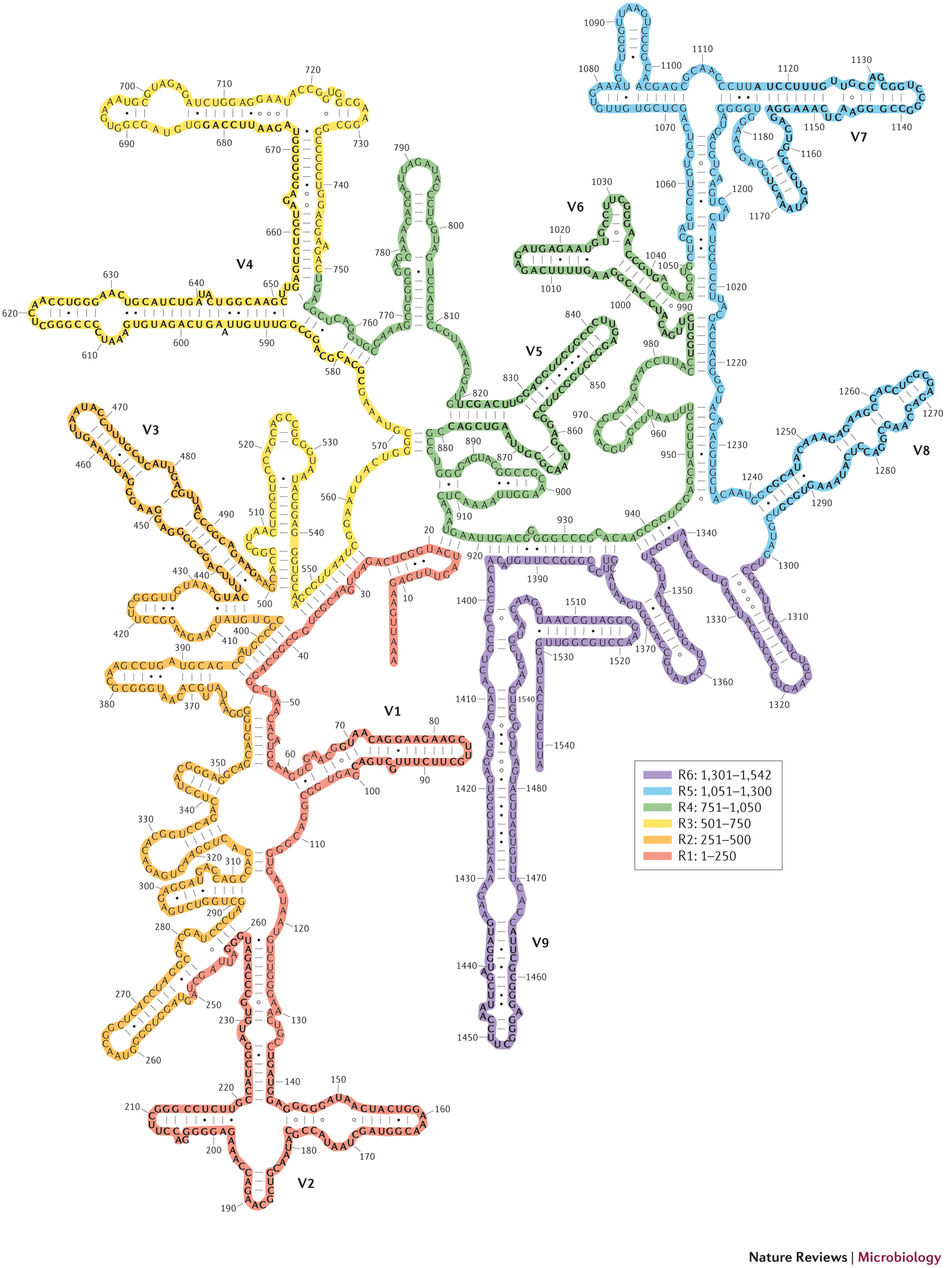
\includegraphics[height=5.5cm, width=5cm]{ribosome.jpg} \\
	\tiny{Yarza, P., et al. Nature Reviews Microbiology 2014}
	\end{columns}

	
	
	\end{frame}
	%-----------------------------------------------------------
	\begin{frame}{Degenerate Primers}
	\begin{columns}
	926 R
	
	\column{0.5\textwidth}
	\begin{block}{Degenerate Primer Example}
	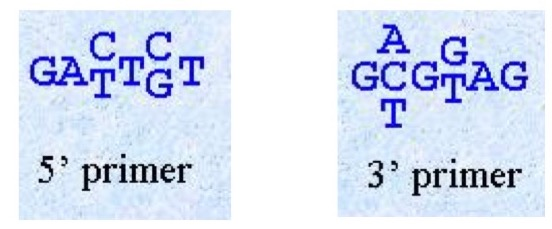
\includegraphics[height=3cm, width=5cm]{CPBS_11_18/primers.jpg}
	\end{block}
	\column{0.5\textwidth}
	\begin{block}{Feature of Degenerate Primers}
	Dual amplification of eukaryotic (18S) and prokaryote (16S)
	\end{block}
	\begin{block}{Universal 16S/18S Primer}
	515F - 806R primer
	\end{block}
	\end{columns}
	\tiny{Caporaso, J.G., et al. PNAS 2011 \\ Wang, Y., et al. PLOS One 2014}

	\end{frame}
	%-----------------------------------------------------------
	\begin{frame}{Objective}
	Develop an optimized pipeline to accurately describe composition of an environmental sample.
	\begin{block}{Methods Testing}
	\begin{itemize}
	\item Standard OTU Picking with expanded database
	\item Error correction with expanded database
	\item Filtering 18S by merging status and parallel processing
	\end{itemize}
	\end{block}
	\end{frame}
	%-----------------------------------------------------------
	\begin{frame}{Simulated Metagenome}
	\center
	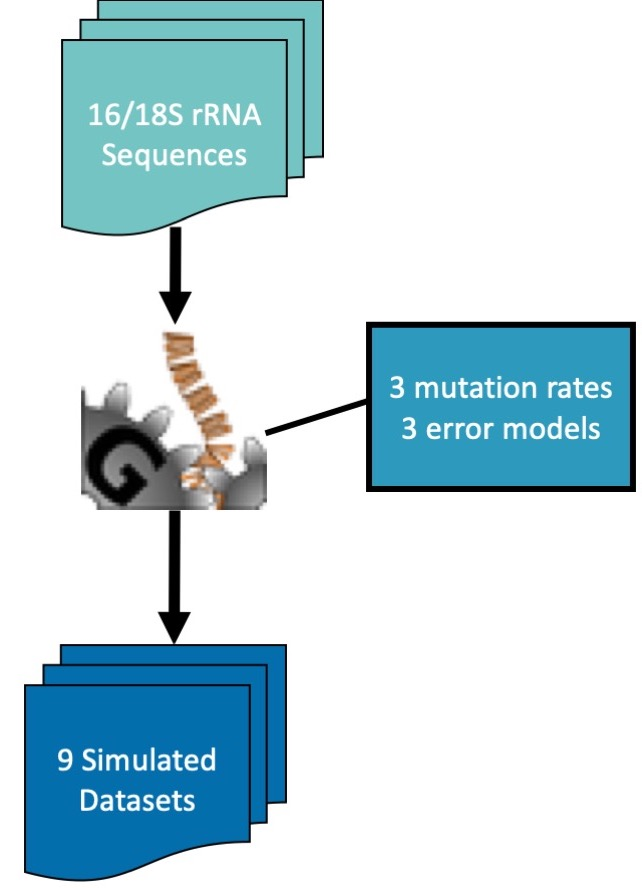
\includegraphics[height=7cm, width=7cm]{CPBS_11_18/simulated.jpg}
	\begin{flushright}
	
	not using mutation, used three different composition
	
	
	\tiny{Pamela Russell \\ Angly, F.E., et al. Nucleic acids research 2012}
	\end{flushright}
	\end{frame}
	%-----------------------------------------------------------
	\begin{frame}{Testing pipelines}
	\vspace{-0.5cm}
	\center
	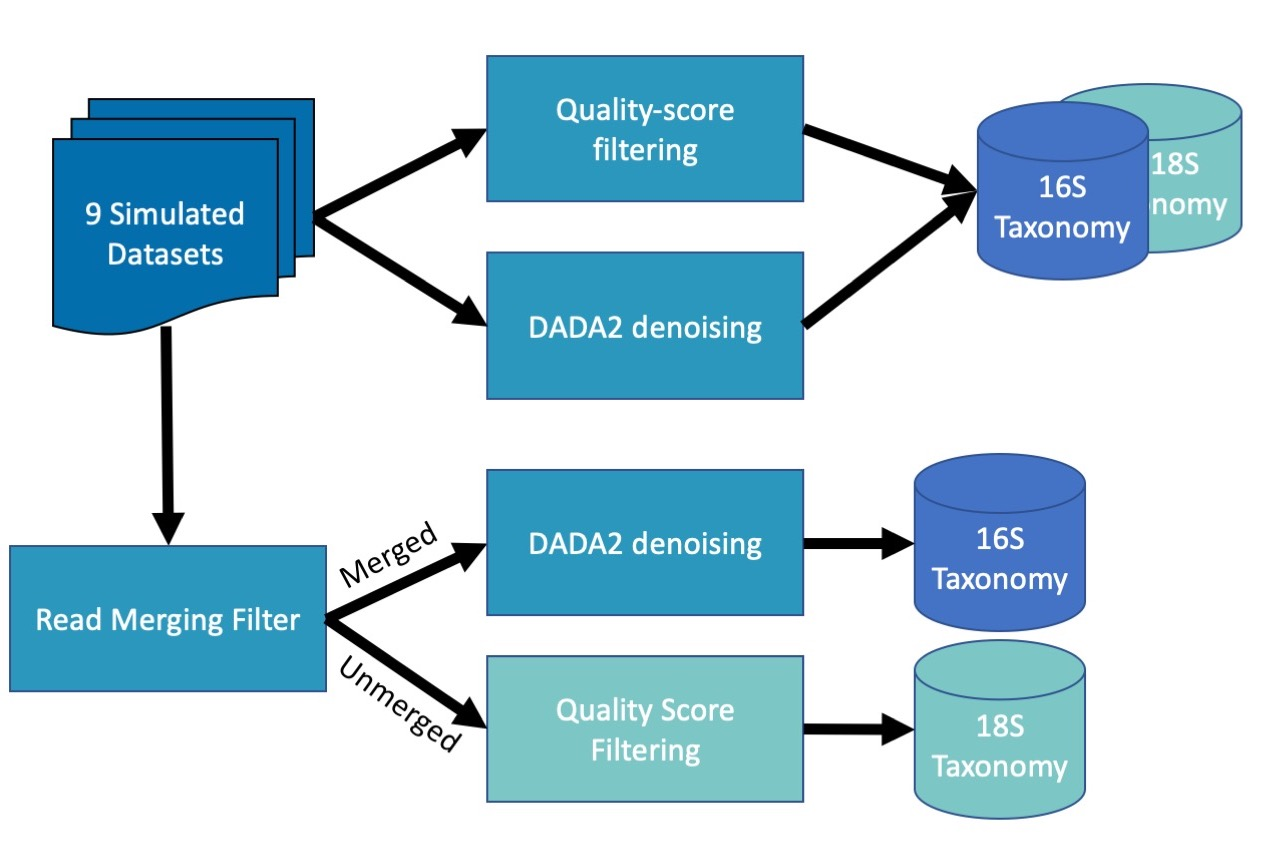
\includegraphics[height=8cm, width=11cm]{CPBS_11_18/duo_pipe.jpg}
	\begin{flushright}
	\tiny{Callahan, B. J., et al. Nature Methods 2016}
	\end{flushright}
	\end{frame}

	
\section{}
\subsection{}
%------------------------------------------------------------------ Outline
	\begin{frame}{Research Update Outline}
	\begin{block}{\textcolor{black!50}{Virulence Factors in Bacteriophages}}
	\textcolor{black!50}{In preperation}
	\end{block}
	
	\begin{block}{Building Up Domains: Lysogenic Host Discovery}
	Incorporated into large collaborative NCBI initative
	\end{block}

	\begin{block}{\textcolor{black!50}{Hybrid Viral Contig Prediction}}
	\textcolor{black!50}{In Preperation}
	\end{block}
	\end{frame}
%------------------------------------------------------------------

	
\section{Hybrid Viral Contig Prediction}
\subsection{}
%-------------------------------------
  \begin{frame}{Metagenomics}
	\begin{columns}
	\column{0.5\textwidth}
	\begin{block}{What is Metagenomics?}
	Unbiased study of all genetic material in a sample
	\end{block}
	\begin{block}{Importance of Metagenomics}
	\begin{itemize}
	\item Functional capabilities of a sample
	\item Species level distinctions
	\item Due to lack of a universal gene marker, phages are studied by metagenomics
	\end{itemize}
	\end{block}
	
	\column{0.5\textwidth}
	
\includegraphics[height=5.5cm, width=5cm]{mosaic.png}
	\end{columns}
	\end{frame}

%-------------------------------------
  \begin{frame}{Methods to Isolate Phages in Metagenomics}
  \begin{block}{Biological Isolations}
  Filtrations and density gradiants to collect small particles
  \end{block}
  \begin{block}{Sequence Similarity}
  Mapping to genomes, BLAST, and Hidden Markov Models
  \end{block}
  \begin{block}{Machine Learning Methods}
  Linear discriminant analysis classier on sequence k-mer profiles
  \end{block}
  \end{frame}
  
  \begin{frame}{Two-Step Hybrid Model}
  Insert Pipeline
  
  \end{frame}
  
  \begin{frame}{Methods}
  HMMs from Earth Virome
  
  Python developed model with standalone operability
  Mycobacterium, Pseudomonas, Lactobacillus
  \end{frame}

\section{}

	\begin{frame}{Concluding Remarks}
	\center
	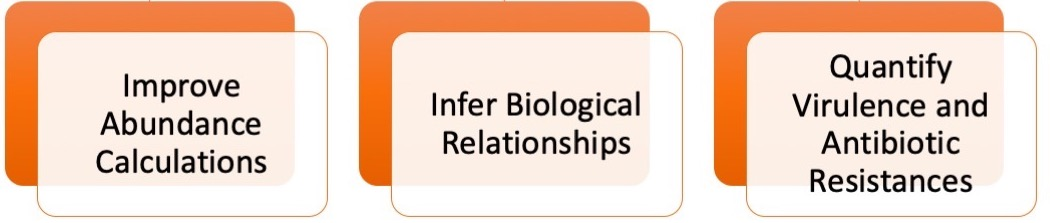
\includegraphics[height=2cm, width=10cm]{goals.jpg}
	\begin{columns}
	\column{0.3\textwidth}
	\begin{block}{DuoBiome}
	Optimized methods to simultaneously explore eukaryotic and prokaryotic communties
	\end{block}
	\column{0.3\textwidth}
	\begin{block}{Hybrid Viral Contig Prediction}
	A hybrid model to identify phage elements in metagenomics and connect them with bacteria
	\end{block}
	\column{0.3\textwidth}
	\begin{block}{Virulence Factors in Phages}
	First quantification of bacterial virulence factors within phage genomes
	\end{block}
	
	\end{columns}
	
	\end{frame}
	
	
	
	
	\begin{frame}{}
	\vspace{1cm}
	{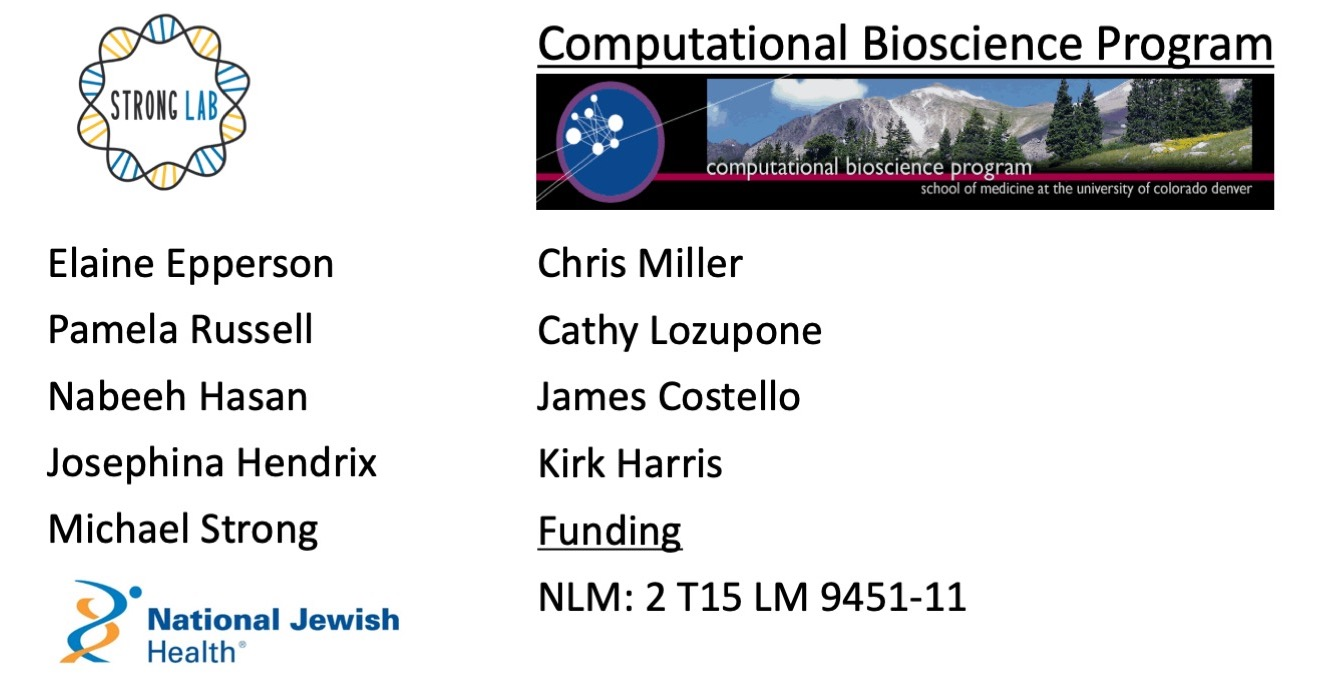
\includegraphics[height=7cm, width=11cm]{acknowledgement.jpg} }
	\end{frame}
	
	
	\begin{frame}{Questions?}
	\center
	Cody Glickman \\ 
\includegraphics[height=2cm, width=2cm]{lablogo.png} \\ cody.glickman@ucdenver.edu \\ \alert{www.github.com/glickmac} \\ www.codyglickman.com
	\end{frame}
	
	%\begin{itemize}
	%\item Prophages in bacterial reference genomes are well annotated
	%\item Location in bacterial reference genome is well annotated
	%\item find prophages in contigs and map contigs to reference.
	
	
\end{document}